% !TEX root =  ../main_manuscript.tex

\section{Methods}
\label{sec:methods}
We start with a short introduction of the PRIAS dataset and the joint modeling framework we will use in our following developments. The PRIAS dataset consists of 5270 AS patients. For each patient, PSA measurements (ng/mL) are scheduled every 3 months for first 2 years and every 6 months thereafter. DRE measurements which are binary with two levels, namely $\mbox{DRE} > \mbox{T1c}$ and $\mbox{DRE} \leq \mbox{T1c}$ \cite{schroder1992tnm}, are scheduled every 6 months. Larger values for PSA and/or larger score for DRE, may indicate cancer progression. Biopsies are scheduled as per the PRIAS protocol (see \hyperref[sec:introduction]{Introduction}). 

\subsection{Joint Model for Time-to-Event and Longitudinal Data}
Let $T_i^*$ denote the true cancer progression time for the $i$-th AS patient. Let $T_i^R$ and $T_i^{R-1}$ denote the time of his latest and second latest biopsies, respectively. Since biopsies are conducted periodically, $T_i^*$ cannot be observed directly and it is only known to fall in an interval $l_i < T_i^* \leq r_i$, where $l_i = T_i^{R-1}, r_i = T_i^R$ if progression is observed at the latest biopsy, and $l_i = T_i^R, r_i=\infty$ if progression is not observed yet. Further let $\boldsymbol{y}_{1i}, \boldsymbol{y}_{2i}$ denote the $n_{1i} \times 1$ and $n_{2i} \times 1$ vectors of the DRE and PSA longitudinal measurements, respectively. For a sample of $n$ patients the observed data is denoted by $\mathcal{D}_n = \{l_i, r_i, \boldsymbol{y}_{1i}, \boldsymbol{y}_{2i}; i = 1, \ldots, n\}$.
\begin{figure}[!htb]
\captionsetup{justification=justified}
\centerline{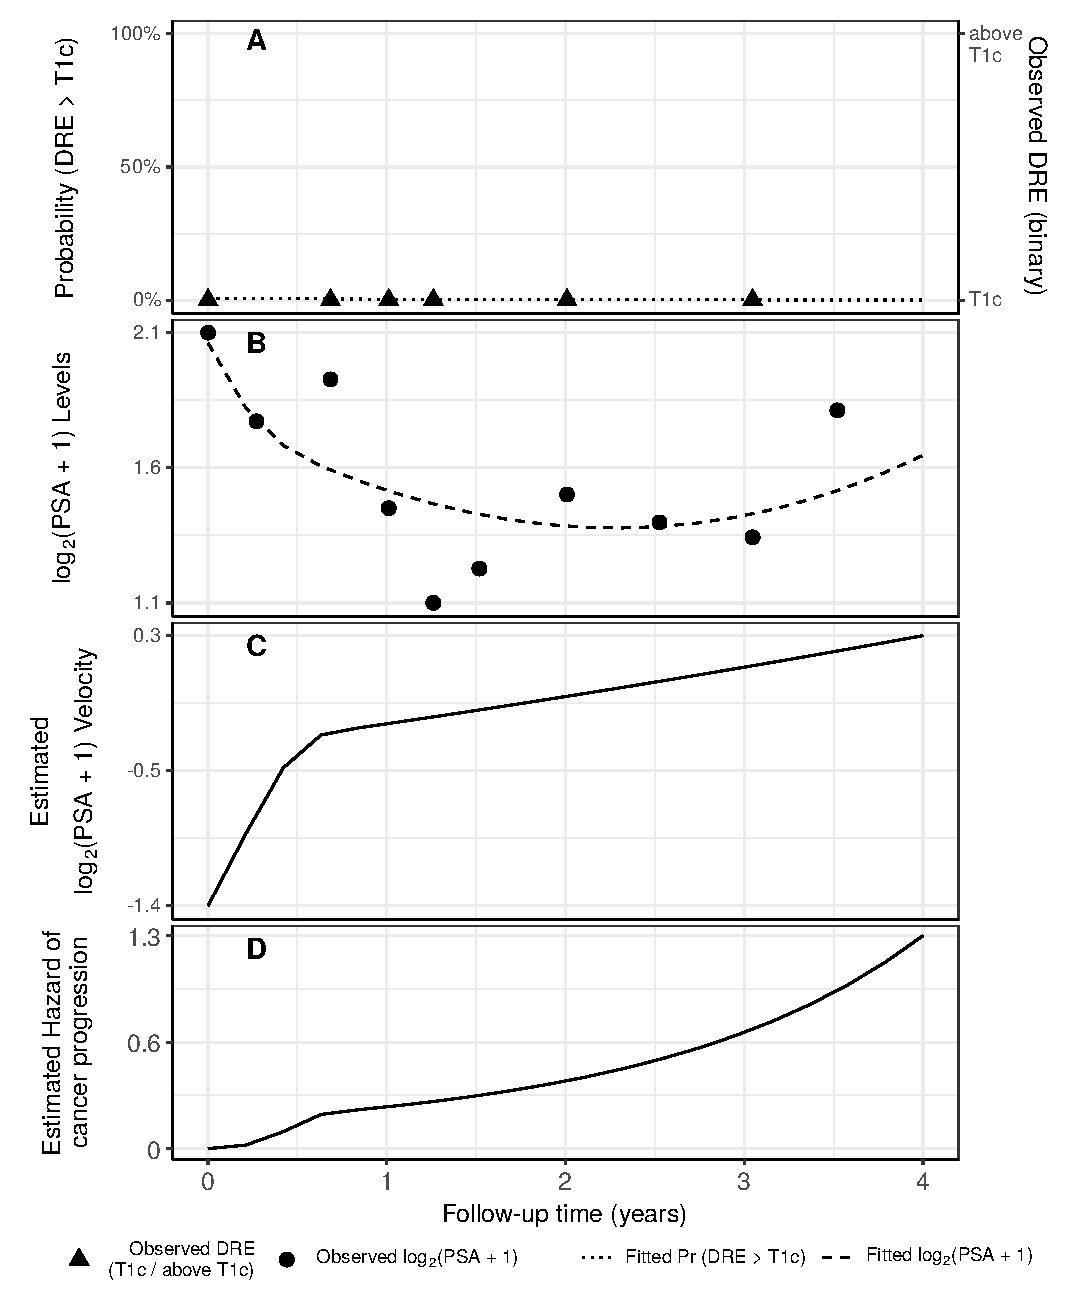
\includegraphics[width=\columnwidth]{images/jmExplanationPlot_1757.eps}}
\caption{Illustration of the joint model fitted to the PRIAS dataset. Panel A shows the fitted $\log_2 \{y_{2i}(t) + 1\}$ velocity (velocity can only be estimated, not observed) over time. Panel B shows the observed and fitted $\log_2 \{y_{2i}(t) + 1\}$ levels. Panel C shows the observed DRE scores and the fitted probability of obtaining a DRE score greater than T1c level. The hazard function shown in Panel D, depends on the fitted log odds of having $\mbox{DRE} > \mbox{T1c}$, and the fitted $\log_2 \{y_{2i}(t) + 1\}$ value and velocity.}
\label{fig:jmExplanationPlot_1757}
\end{figure}

The patient-specific PSA and DRE measurements over time are modeled using a generalized linear mixed effects model. For the $i$-th patient, the sub-model for DRE is given by:
\begin{equation}
\label{eq:long_model_dre}
\begin{aligned}
    \mbox{logit} \big[\mbox{Pr}\{y_{1i}(t) > \mbox{T1c}\}\big] &= \beta_{01} + b_{01i} + (\beta_{11} + b_{11i}) t\\
    &+ \beta_{21} (\mbox{Age}_i-70) + \beta_{31} (\mbox{Age}_i-70)^2\\ 
    \end{aligned}
\end{equation}
where, $\mbox{Age}_i$ is the age of the $i$-th patient at the time of inclusion in AS, $\beta_{\cdot1}$ are the fixed effect parameters, and $b_{\cdot1i}$ are the random effect parameters. An example model fit for DRE is shown in Panel C of Figure \ref{fig:jmExplanationPlot_1757}. For the $i$-th patient, the sub-model for PSA is given by:
\begin{equation}
\label{eq:long_model_psa}
\begin{aligned}
    \log_2 \big\{y_{2i}(t) + 1\big\} &= \beta_{02} + b_{02i} + \sum_{k=1}^4 (\beta_{k2} + b_{k2i})  B_k(t,\mathcal{K})\\ 
    &+ \beta_{52} (\mbox{Age}_i-70) + \beta_{62} (\mbox{Age}_i-70)^2 + \varepsilon_{2i}(t),
    \end{aligned}
\end{equation}
where, $B_k(t, \mathcal{K})$ denotes the $k$-th basis function of a B-spline with three internal knots at $\mathcal{K} = \{0.1, 0.7, 4\}$ years, and boundary knots at 0 and 5.42 years (0.95 quantile of the observed follow-up times). The fixed effects parameters are denoted by $\beta_{\cdot2}$ and random effects are denoted by $b_{\cdot2i}$. The error $\varepsilon_{2i}(t)$ is assumed to be t-distributed with three degrees of freedom and scale $\sigma$ (see Web Appendix C.1), and is independent of the random effects $b_{\cdot2i}$. An example model fit for PSA is shown in Panel B of Figure \ref{fig:jmExplanationPlot_1757}. To account for the association between the DRE and PSA measurements, we link their corresponding random effects. More specifically, the complete vector of random effects $\boldsymbol{b}_i = (b_{\cdot1i}, b_{\cdot2i})^T$ is assumed to follow a multivariate normal distribution with mean zero and variance-covariance matrix $\boldsymbol{D}$.

To model the impact of DRE and PSA measurements on the risk of cancer progression, we use a relative risk sub-model. More specifically, the hazard of cancer progression $h_i(t)$ at a time $t$ is given by:
\begin{equation}
\label{eq:rel_risk_model}
\begin{aligned}
    h_i(t) &= h_0(t) \exp\Big(\alpha_{11} \mbox{logit} \big[\mbox{Pr}\{y_{1i}(t) > \mbox{T1c}\}\big]\\
    &+ \alpha_{21} E\big[\log_2 \big\{y_{2i}(t) + 1\big\}\big] + \alpha_{22} \frac{\mathrm{d}{E\big[\log_2 \big\{y_{2i}(t) + 1\big\}\big]}}{\mathrm{d}{t}}\\
    &+ \gamma_1 (\mbox{Age}_i-70) + \gamma_2 (\mbox{Age}_i-70)^2 \Big),
    \end{aligned}
\end{equation}
where, $\gamma_1$, $\gamma_2$ are the coefficients for the effect of Age. The parameter $\alpha_{11}$models the impact of log odds of having $\mbox{DRE} > \mbox{T1c}$ on the hazard of cancer progression. The impact of PSA on cancer progression is modeled in two ways, namely at any time $t$ the effect of the instantaneous underlying value of PSA $E[\log_2 \{y_{2i}(t) + 1\}]$ is given by $\alpha_{21}$, and the effect of the instantaneous underlying velocity (panel A in Figure \ref{fig:jmExplanationPlot_1757}) of PSA $\mathrm{d}{E[\log_2 \{y_{2i}(t) + 1\}]}/\mathrm{d}{t}$ is given by $\alpha_{22}$. Lastly, $h_0(t)$ is the baseline hazard at time t, and is modeled flexibly using P-splines. An example fitted hazard is shown in Panel D of Figure \ref{fig:jmExplanationPlot_1757}.  The detailed specification of the baseline hazard, and parameter estimation using the Bayesian approach are presented in Web Appendix A of the supplementary material.


\subsection{Personalized Decisions for Biopsy During Follow-up Visit}
\label{subsec:pers_decision_making}
We intend to use the joint model fitted to the PRIAS dataset, to personalize the decision of conducting biopsies at follow-up visits. To this end, let us assume that a decision of conducting a biopsy is to be made for a new patient $j$, who is not present in the PRIAS dataset. Let $t$ be the time of his latest biopsy, and $s$ denotes the current follow-up visit time. Let $\mathcal{Y}_{1j}(s)$ and $\mathcal{Y}_{2j}(s)$ denote the vector of all DRE and PSA measurements taken up to the current visit, respectively. We first combine all the observed information to yield a posterior predictive distribution $g(T^*_j)$ of the time of cancer progression $T^*_j$. It is given by:
\begin{equation*}
\label{eq:post_pred_dist}
\begin{aligned}
g(T^*_j) &= p\big\{T^*_j \mid T^*_j > t, \mathcal{Y}_{1j}(s), \mathcal{Y}_{2j}(s), \mathcal{D}_n\big\}\\
&= \int \int p\big(T^*_j \mid T^*_j > t, \boldsymbol{b}_j, \boldsymbol{\theta}\big)\\
&\times p\big\{\boldsymbol{b}_j \mid T^*_j>t, \mathcal{Y}_{1j}(s), \mathcal{Y}_{2j}(s), \boldsymbol{\theta}\big\}p\big(\boldsymbol{\theta} \mid \mathcal{D}_n\big) \mathrm{d} \boldsymbol{b}_j \mathrm{d} \boldsymbol{\theta}.
\end{aligned}
\end{equation*}
The distribution $g(T^*_j)$ is unique for each patient, and updates at every follow-up visit. It depends on the historical data of the patient via the posterior distribution of the random effects $\boldsymbol{b}_j$. 

To make personalized decisions for biopsies, we utilize the personalized distribution $g(T^*_j)$.
From a patient or doctor's perspective the decision of conducting biopsy at a follow-up visit should account for the patient's risk of having a cancer progression $R_j(s \mid t, s)$ up to the current visit since the latest biopsy. We estimate this risk from the distribution $g(T^*_j)$ \cite{rizopoulos2011dynamic}. The risk is given by:
\begin{equation*}
\label{eq:dynamic_risk_prob}
R_j(s \mid t, s) = \mbox{Pr}\big\{T^*_j \leq s \mid T^*_j > t, \mathcal{Y}_{1j}(s), \mathcal{Y}_{2j}(s) \mathcal{D}_n\big\}.
\end{equation*}
We propose to conduct a biopsy at a follow-up visit if this risk is higher than a certain threshold $0 \leq \kappa \leq 1$, as illustrated in Figure \ref{fig:dynRiskPlot_2340}. While this approach is considerate about a patient's apprehensions for his risk of cancer progression, choosing too a small a threshold may lead to too many biopsies. To obtain an insight on the impact of thresholds, we evaluate a small risk of 5\% and a slightly higher risk of 15\% in this work.
\begin{figure}[!htb]
\captionsetup{justification=justified}
\centerline{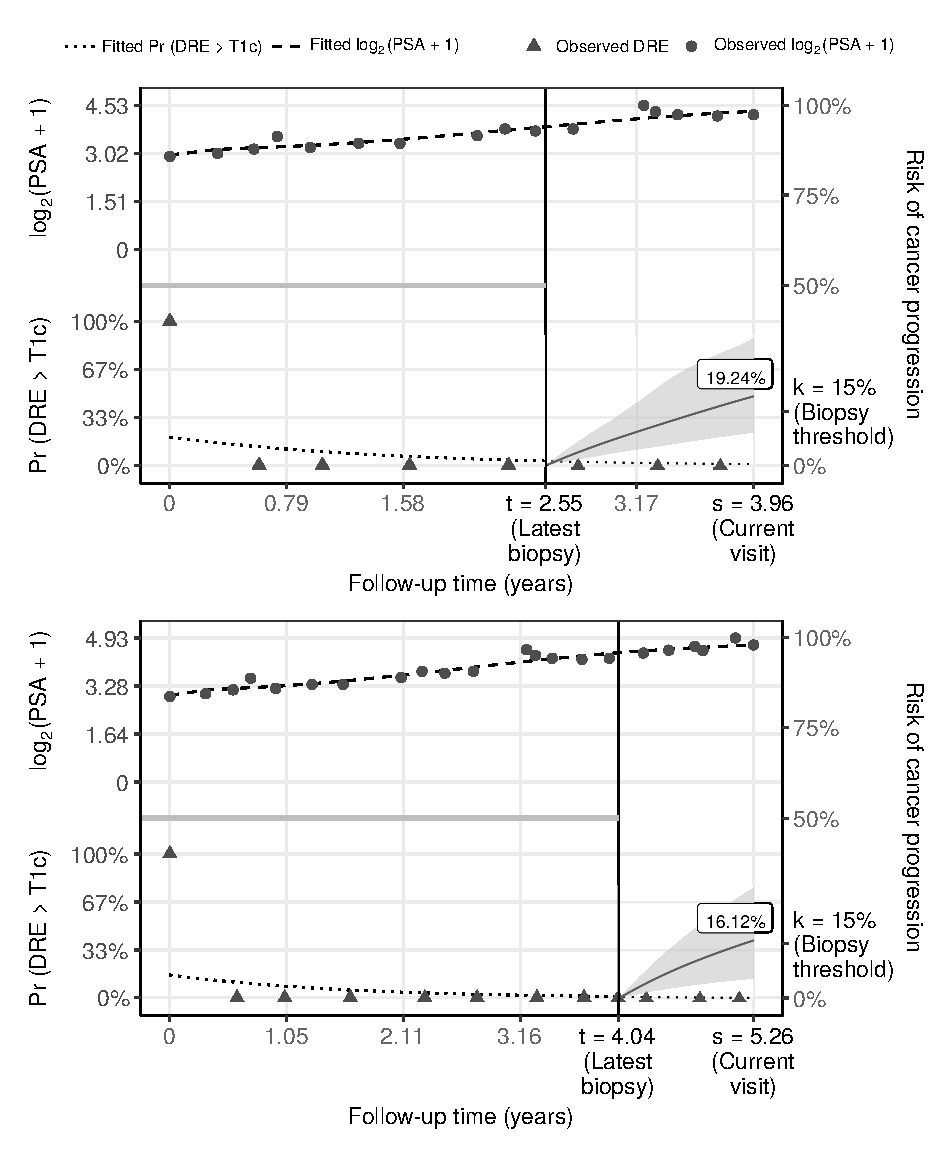
\includegraphics[width=\columnwidth]{images/dynRiskPlot_2340.eps}}
\caption{Illustration of personalized decision making for a patient at two different follow-up visits, namely $s=3.96$ years in top panel and $s=5.26$ years in bottom panel. The latest biopsy of the patient at which cancer progression was not detected is at $t=2.55$ years in top panel and $t=4.04$ in bottom panel. The risk of cancer progression, estimated on the basis of the fitted PSA and DRE profiles, and the latest biopsy,  is shown in the right sub-panel with the 95\% credible interval (shaded region). The risk at the current visit is estimated to be 19.24\% in top panel and 16.12\% in bottom panel. Since the risk is higher than the biopsy threshold $\kappa=15\%$, a biopsy will be scheduled at the current visit in both panels.}
\label{fig:dynRiskPlot_2340}
\end{figure}

A drawback of fixed thresholds is that they do not vary as per the general cancer progression rates of AS patients at a certain visit time. In this regard, we propose to select a threshold on the basis of its ability to discriminate between patients who obtain cancer progression versus others. More specifically, given the time $t$ of the latest biopsy we propose to choose a $\kappa$ for which a binary classification accuracy measure \citep{lopez2014optimalcutpoints}, discriminating between patients obtaining progression versus others, is maximized. In joint models, a patient $j$ is predicted to have progression in the time period up to current visit since last biopsy $(t, s]$, if $R_j(s \mid t,s) > \kappa$, or a control if $R_j(s \mid t,s) \leq \kappa$ \cite{rizopoulosJMbayes, landmarking2017}. Since we are interested in detecting progression, we choose $\mbox{F}_1$ score as the classification accuracy measure. It combines both time dependent true positive rate (TPR) and positive predictive value (PPV) \cite{landmarking2017}, and is defined as:
\begin{align*}
\mbox{F}_1(t,  s, \kappa) &= 2\frac{\mbox{TPR}(t,  s, \kappa)\ \mbox{PPV}(t,  s, \kappa)}{\mbox{TPR}(t,  s, \kappa) + \mbox{PPV}(t,  s, \kappa)},\\
\mbox{TPR}(t,  s, \kappa) &= \mbox{Pr}\big\{R_j(s \mid t,s) > \kappa \mid t < T^*_j \leq s\big\},\\
\mbox{PPV}(t,  s, \kappa) &= \mbox{Pr}\big\{t < T^*_j \leq s \mid R_j(s \mid t,s) > \kappa \big\}.
\end{align*}
Since a high $\mbox{F}_1$ score is desired, the corresponding value of $\kappa$ is $\argmax_{\kappa} \mbox{F}_1(t, s, \kappa)$.

\subsection{Simulation Study}
Although the personalized decision making approach is motivated by the PRIAS study, it is not possible to evaluate it on the PRIAS dataset. This is due to the fact that the PRIAS patients have already had their biopsies as per the PRIAS protocol. In addition, the true time of cancer progression is interval or right censored for all patients, making it impossible to correctly estimate the delay in detection of cancer progression due to a particular schedule. To this end, we conduct an extensive simulation study to compare personalized, PRIAS and annual schedules. For a realistic comparison, we utilize an exact replica of the population of the PRIAS patients. The simulation study follow-up period of 10 years also similar to the that of PRIAS study.

To simulate a replica of the population of the PRIAS patients, we generate the PSA and DRE profiles, and distribution of cancer progression times for hypothetical patients using the posterior distribution of the parameters of the joint model fitted to the PRIAS dataset. From this population, we first sample 500 datasets with 1000 patients each. We generate a true cancer progression time for each of the patients, and then sample a set of PSA and DRE measurements at the same time points as given in PRIAS protocol. We then split the dataset into a training (750 patients) and a test (250 patients) part, and generate a random and non‐informative censoring time for the training patients. We next fit a joint model of the specification given in Equation (\ref{eq:long_model_dre}), (\ref{eq:long_model_psa}) and (\ref{eq:rel_risk_model}) to each of the 500 training datasets and obtain MCMC samples from the 500 sets of the posterior distribution of the parameters. Using these fitted joint models, we obtain the posterior predictive distribution of time of cancer progression for each of the 500$\times$250 test patients at each of their visits. While maintaining a gap of 1 year between consecutive biopsies, individually for each patient at each follow-up visit we make the decision of (not) conducting a biopsy as per the methodology described in \hyperref[subsec:pers_decision_making]{Personalized Decisions for Biopsy}. This results into an entire personalized schedule for each patient.

In this simulation study, for every test patient we conduct hypothetical biopsies. One biopsy is conducted for all patients at the beginning of the AS program and another one is conducted at the end of the follow-up period at 10 years. The rest of the biopsies are scheduled using the following methods: (abbreviated names in parenthesis): biopsy every year (Annual), biopsy as per PRIAS protocol (PRIAS), personalized biopsy using a risk threshold of 5\% (Risk: 5\%), personalized biopsy using a risk threshold of 15\% (Risk: 15\%), and personalized biopsy using a risk threshold chosen on the basis of progression history of patients from the training dataset (Risk: $\mbox{F}_1$). We compare the resulting biopsy schedules on two measures, namely the number of biopsies they schedule and the delay in detection of cancer progression incurred due the schedule. We define the delay as the difference between the time of the biopsy on which cancer progression is detected and the true time of cancer progression. Ideal numbers for these two measures are 1 biopsy and 0 years of delay.